\documentclass[border=3pt]{standalone}
\usepackage{fontspec}
\setmainfont{Latin Modern Roman}
\usepackage{pgfplots}
\pgfplotsset{compat=1.18}
\usetikzlibrary{arrows.meta,calc,positioning,shapes.geometric}
\definecolor{forest}{HTML}{346E57}
\definecolor{sage}{HTML}{E8EFEA}
\definecolor{clay}{HTML}{B77E60}
\definecolor{gray}{HTML}{718078}
\definecolor{rule}{HTML}{B7C3BA}
\definecolor{ink}{HTML}{000000}
\begin{document}
\hyphenpenalty=10000\exhyphenpenalty=10000
\fontsize{10}{12}\selectfont
\renewcommand{\small}{\fontsize{9}{11}\selectfont}
\renewcommand{\scriptsize}{\fontsize{8}{10}\selectfont}
\resizebox{16cm}{!}{%
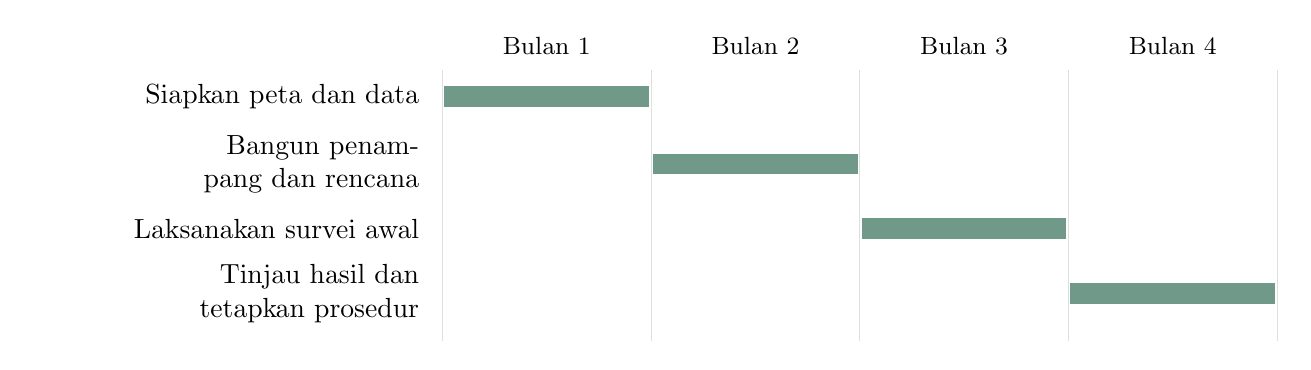
\begin{tikzpicture}[x=1cm,y=1cm]
\node[anchor=north east,text width=4.9cm,align=right,inner sep=2pt] (task0) at (-.22,0) {Siapkan peta dan data};
\coordinate (row0) at (0,0 |- task0.center);
\fill[forest!70] ($(row0)+(0.025,-.13)$) rectangle ($(row0)+(2.625,.13)$);
\node[anchor=north east,text width=4.9cm,align=right,inner sep=2pt] (task1) at ($(task0.south east)+(0,-.18)$) {Bangun penampang dan rencana};
\coordinate (row1) at (0,0 |- task1.center);
\fill[forest!70] ($(row1)+(2.675,-.13)$) rectangle ($(row1)+(5.2749999999999995,.13)$);
\node[anchor=north east,text width=4.9cm,align=right,inner sep=2pt] (task2) at ($(task1.south east)+(0,-.18)$) {Laksanakan survei awal};
\coordinate (row2) at (0,0 |- task2.center);
\fill[forest!70] ($(row2)+(5.325,-.13)$) rectangle ($(row2)+(7.924999999999999,.13)$);
\node[anchor=north east,text width=4.9cm,align=right,inner sep=2pt] (task3) at ($(task2.south east)+(0,-.18)$) {Tinjau hasil dan tetapkan prosedur};
\coordinate (row3) at (0,0 |- task3.center);
\fill[forest!70] ($(row3)+(7.975,-.13)$) rectangle ($(row3)+(10.575,.13)$);
\coordinate (gridBottom) at ($(task3.south)+(0,-.16)$);
\node[font=\small,text width=2.57cm,align=center,anchor=south] at (1.325,.18) {Bulan 1};
\draw[rule!50,line width=.3pt] (0.0,.1) -- (0.0,0 |- gridBottom);
\node[font=\small,text width=2.57cm,align=center,anchor=south] at (3.9749999999999996,.18) {Bulan 2};
\draw[rule!50,line width=.3pt] (2.65,.1) -- (2.65,0 |- gridBottom);
\node[font=\small,text width=2.57cm,align=center,anchor=south] at (6.625,.18) {Bulan 3};
\draw[rule!50,line width=.3pt] (5.3,.1) -- (5.3,0 |- gridBottom);
\node[font=\small,text width=2.57cm,align=center,anchor=south] at (9.275,.18) {Bulan 4};
\draw[rule!50,line width=.3pt] (7.949999999999999,.1) -- (7.949999999999999,0 |- gridBottom);
\draw[rule!50,line width=.3pt] (10.6,.1) -- (10.6,0 |- gridBottom);
\end{tikzpicture}
}

\end{document}
